\begin{frame}{Les associations des verbes \lexi{-er}}
  \centering
  \begin{itemize}
    \item Des mots associés à \lexi{regarder}
    \item[$\to$] la télé, un film, le tableau
    \item[] \tinygloss{Some words associated with \lexi{regarder}}
    \item[] \tinygloss{$\to$ la télé, un film, le tableau}
  \end{itemize}
\end{frame}

\begin{frame}{Les associations des verbes \lexi{-er}}
  \centering
  écouter

  \uncover<2->{
    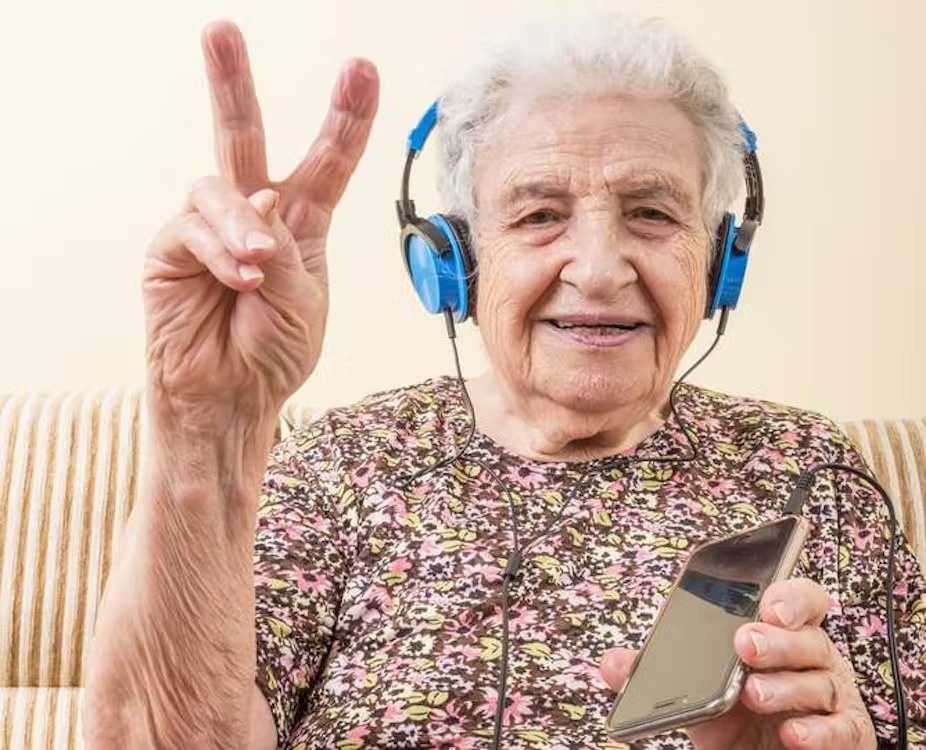
\includegraphics[scale=0.2]{ecouter.jpg}
  }
\end{frame}

\begin{frame}{Les associations des verbes \lexi{-er}}
  \centering
  jouer

  \uncover<2->{
    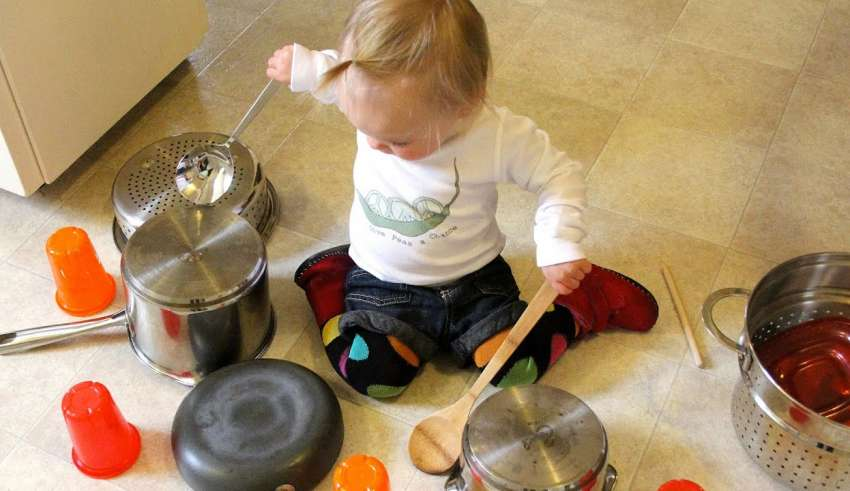
\includegraphics[scale=0.4]{jouer.jpg}
  }
\end{frame}

\begin{frame}{Les associations des verbes \lexi{-er}}
  \centering
  préparer

  \uncover<2->{
    \includegraphics[scale=1]{préparer.jpg}
  }
\end{frame}

\begin{frame}{Les associations des verbes \lexi{-er}}
  \centering
  parler

  \uncover<2->{
    
\includegraphics[scale=0.25]{parler.jpg}
  }
\end{frame}

% \begin{frame}{Les associations des verbes \lexi{-er}}
%   \centering
%   travailler

%   \uncover<2->{
%     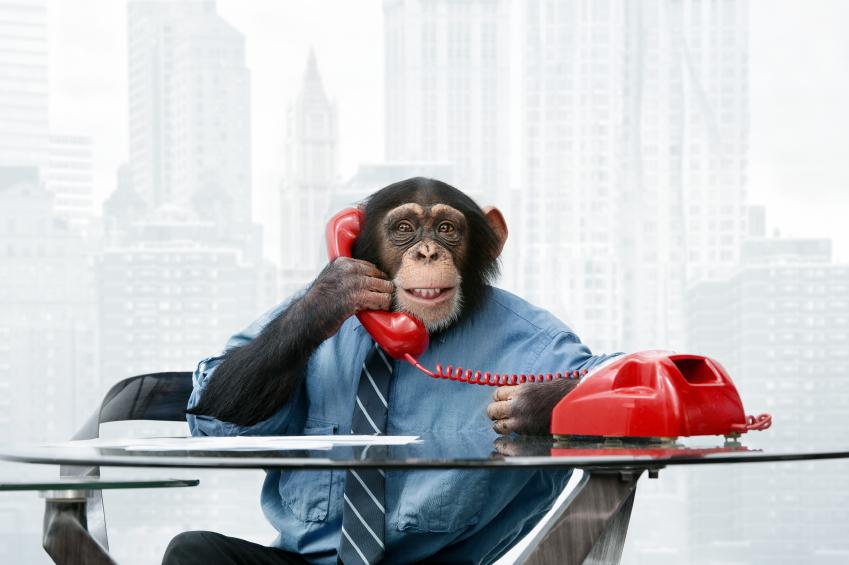
\includegraphics[scale=0.75]{travailler.jpg}
%   }
% \end{frame}

% \begin{frame}{Les associations des verbes \lexi{-er}}
%   \begin{columns}
%     \column{0.5\textwidth}
%       \begin{center}
%         inviter
%       \end{center}
%     \column{0.5\textwidth}
%       \begin{center}
%         \uncover<2->{
%           
\includegraphics[scale=0.37]{inviter.jpg}
%         }
%       \end{center}
%   \end{columns}
% \end{frame}